\documentclass[1p]{elsarticle_modified}
%\bibliographystyle{elsarticle-num}

%\usepackage[colorlinks]{hyperref}
%\usepackage{abbrmath_seonhwa} %\Abb, \Ascr, \Acal ,\Abf, \Afrak
\usepackage{amsfonts}
\usepackage{amssymb}
\usepackage{amsmath}
\usepackage{amsthm}
\usepackage{scalefnt}
\usepackage{amsbsy}
\usepackage{kotex}
\usepackage{caption}
\usepackage{subfig}
\usepackage{color}
\usepackage{graphicx}
\usepackage{xcolor} %% white, black, red, green, blue, cyan, magenta, yellow
\usepackage{float}
\usepackage{setspace}
\usepackage{hyperref}

\usepackage{tikz}
\usetikzlibrary{arrows}

\usepackage{multirow}
\usepackage{array} % fixed length table
\usepackage{hhline}

%%%%%%%%%%%%%%%%%%%%%
\makeatletter
\renewcommand*\env@matrix[1][\arraystretch]{%
	\edef\arraystretch{#1}%
	\hskip -\arraycolsep
	\let\@ifnextchar\new@ifnextchar
	\array{*\c@MaxMatrixCols c}}
\makeatother %https://tex.stackexchange.com/questions/14071/how-can-i-increase-the-line-spacing-in-a-matrix
%%%%%%%%%%%%%%%

\usepackage[normalem]{ulem}

\newcommand{\msout}[1]{\ifmmode\text{\sout{\ensuremath{#1}}}\else\sout{#1}\fi}
%SOURCE: \msout is \stkout macro in https://tex.stackexchange.com/questions/20609/strikeout-in-math-mode

\newcommand{\cancel}[1]{
	\ifmmode
	{\color{red}\msout{#1}}
	\else
	{\color{red}\sout{#1}}
	\fi
}

\newcommand{\add}[1]{
	{\color{blue}\uwave{#1}}
}

\newcommand{\replace}[2]{
	\ifmmode
	{\color{red}\msout{#1}}{\color{blue}\uwave{#2}}
	\else
	{\color{red}\sout{#1}}{\color{blue}\uwave{#2}}
	\fi
}

\newcommand{\Sol}{\mathcal{S}} %segment
\newcommand{\D}{D} %diagram
\newcommand{\A}{\mathcal{A}} %arc


%%%%%%%%%%%%%%%%%%%%%%%%%%%%%5 test

\def\sl{\operatorname{\textup{SL}}(2,\Cbb)}
\def\psl{\operatorname{\textup{PSL}}(2,\Cbb)}
\def\quan{\mkern 1mu \triangleright \mkern 1mu}

\theoremstyle{definition}
\newtheorem{thm}{Theorem}[section]
\newtheorem{prop}[thm]{Proposition}
\newtheorem{lem}[thm]{Lemma}
\newtheorem{ques}[thm]{Question}
\newtheorem{cor}[thm]{Corollary}
\newtheorem{defn}[thm]{Definition}
\newtheorem{exam}[thm]{Example}
\newtheorem{rmk}[thm]{Remark}
\newtheorem{alg}[thm]{Algorithm}

\newcommand{\I}{\sqrt{-1}}
\begin{document}

%\begin{frontmatter}
%
%\title{Boundary parabolic representations of knots up to 8 crossings}
%
%%% Group authors per affiliation:
%\author{Yunhi Cho} 
%\address{Department of Mathematics, University of Seoul, Seoul, Korea}
%\ead{yhcho@uos.ac.kr}
%
%
%\author{Seonhwa Kim} %\fnref{s_kim}}
%\address{Center for Geometry and Physics, Institute for Basic Science, Pohang, 37673, Korea}
%\ead{ryeona17@ibs.re.kr}
%
%\author{Hyuk Kim}
%\address{Department of Mathematical Sciences, Seoul National University, Seoul 08826, Korea}
%\ead{hyukkim@snu.ac.kr}
%
%\author{Seokbeom Yoon}
%\address{Department of Mathematical Sciences, Seoul National University, Seoul, 08826,  Korea}
%\ead{sbyoon15@snu.ac.kr}
%
%\begin{abstract}
%We find all boundary parabolic representation of knots up to 8 crossings.
%
%\end{abstract}
%\begin{keyword}
%    \MSC[2010] 57M25 
%\end{keyword}
%
%\end{frontmatter}

%\linenumbers
%\tableofcontents
%
\newcommand\colored[1]{\textcolor{white}{\rule[-0.35ex]{0.8em}{1.4ex}}\kern-0.8em\color{red} #1}%
%\newcommand\colored[1]{\textcolor{white}{ #1}\kern-2.17ex	\textcolor{white}{ #1}\kern-1.81ex	\textcolor{white}{ #1}\kern-2.15ex\color{red}#1	}

{\Large $\underline{12a_{0539}~(K12a_{0539})}$}

\setlength{\tabcolsep}{10pt}
\renewcommand{\arraystretch}{1.6}
\vspace{1cm}\begin{tabular}{m{100pt}>{\centering\arraybackslash}m{274pt}}
\multirow{5}{120pt}{
	\centering
	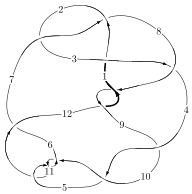
\includegraphics[width=112pt]{../../../GIT/diagram.site/Diagrams/png/1340_12a_0539.png}\\
\ \ \ A knot diagram\footnotemark}&
\allowdisplaybreaks
\textbf{Linearized knot diagam} \\
\cline{2-2}
 &
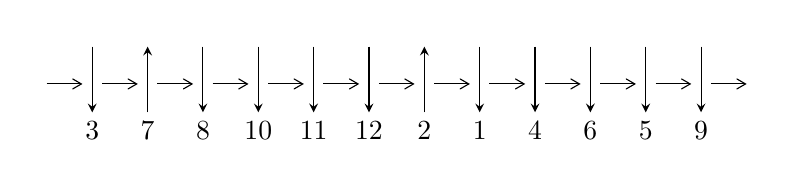
\begin{tikzpicture}[x=20pt, y=17pt]
	% nodes
	\node (C0) at (0, 0) {};
	\node (C1) at (1, 0) {};
	\node (C1U) at (1, +1) {};
	\node (C1D) at (1, -1) {3};

	\node (C2) at (2, 0) {};
	\node (C2U) at (2, +1) {};
	\node (C2D) at (2, -1) {7};

	\node (C3) at (3, 0) {};
	\node (C3U) at (3, +1) {};
	\node (C3D) at (3, -1) {8};

	\node (C4) at (4, 0) {};
	\node (C4U) at (4, +1) {};
	\node (C4D) at (4, -1) {10};

	\node (C5) at (5, 0) {};
	\node (C5U) at (5, +1) {};
	\node (C5D) at (5, -1) {11};

	\node (C6) at (6, 0) {};
	\node (C6U) at (6, +1) {};
	\node (C6D) at (6, -1) {12};

	\node (C7) at (7, 0) {};
	\node (C7U) at (7, +1) {};
	\node (C7D) at (7, -1) {2};

	\node (C8) at (8, 0) {};
	\node (C8U) at (8, +1) {};
	\node (C8D) at (8, -1) {1};

	\node (C9) at (9, 0) {};
	\node (C9U) at (9, +1) {};
	\node (C9D) at (9, -1) {4};

	\node (C10) at (10, 0) {};
	\node (C10U) at (10, +1) {};
	\node (C10D) at (10, -1) {6};

	\node (C11) at (11, 0) {};
	\node (C11U) at (11, +1) {};
	\node (C11D) at (11, -1) {5};

	\node (C12) at (12, 0) {};
	\node (C12U) at (12, +1) {};
	\node (C12D) at (12, -1) {9};
	\node (C13) at (13, 0) {};

	% arrows
	\draw[->,>={angle 60}]
	(C0) edge (C1) (C1) edge (C2) (C2) edge (C3) (C3) edge (C4) (C4) edge (C5) (C5) edge (C6) (C6) edge (C7) (C7) edge (C8) (C8) edge (C9) (C9) edge (C10) (C10) edge (C11) (C11) edge (C12) (C12) edge (C13) ;	\draw[->,>=stealth]
	(C1U) edge (C1D) (C2D) edge (C2U) (C3U) edge (C3D) (C4U) edge (C4D) (C5U) edge (C5D) (C6U) edge (C6D) (C7D) edge (C7U) (C8U) edge (C8D) (C9U) edge (C9D) (C10U) edge (C10D) (C11U) edge (C11D) (C12U) edge (C12D) ;
	\end{tikzpicture} \\
\hhline{~~} \\& 
\textbf{Solving Sequence} \\ \cline{2-2} 
 &
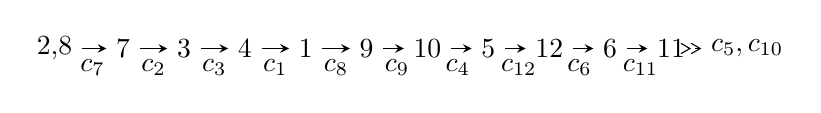
\begin{tikzpicture}[x=22pt, y=7pt]
	% node
	\node (A0) at (-1/8, 0) {2,8};
	\node (A1) at (1, 0) {7};
	\node (A2) at (2, 0) {3};
	\node (A3) at (3, 0) {4};
	\node (A4) at (4, 0) {1};
	\node (A5) at (5, 0) {9};
	\node (A6) at (6, 0) {10};
	\node (A7) at (7, 0) {5};
	\node (A8) at (8, 0) {12};
	\node (A9) at (9, 0) {6};
	\node (A10) at (10, 0) {11};
	\node (C1) at (1/2, -1) {$c_{7}$};
	\node (C2) at (3/2, -1) {$c_{2}$};
	\node (C3) at (5/2, -1) {$c_{3}$};
	\node (C4) at (7/2, -1) {$c_{1}$};
	\node (C5) at (9/2, -1) {$c_{8}$};
	\node (C6) at (11/2, -1) {$c_{9}$};
	\node (C7) at (13/2, -1) {$c_{4}$};
	\node (C8) at (15/2, -1) {$c_{12}$};
	\node (C9) at (17/2, -1) {$c_{6}$};
	\node (C10) at (19/2, -1) {$c_{11}$};
	\node (A11) at (45/4, 0) {$c_{5},c_{10}$};

	% edge
	\draw[->,>=stealth]	
	(A0) edge (A1) (A1) edge (A2) (A2) edge (A3) (A3) edge (A4) (A4) edge (A5) (A5) edge (A6) (A6) edge (A7) (A7) edge (A8) (A8) edge (A9) (A9) edge (A10) ;
	\draw[->>,>={angle 60}]	
	(A10) edge (A11);
\end{tikzpicture} \\ 

\end{tabular} \\

\footnotetext{
The image of knot diagram is generated by the software ``\textbf{Draw programme}" developed by Andrew Bartholomew(\url{http://www.layer8.co.uk/maths/draw/index.htm\#Running-draw}), where we modified some parts for our purpose(\url{https://github.com/CATsTAILs/LinksPainter}).
}\phantom \\ \newline 
\centering \textbf{Ideals for irreducible components\footnotemark of $X_{\text{par}}$} 
 
\begin{align*}
I^u_{1}&=\langle 
u^{72}- u^{71}+\cdots+2 u-1\rangle \\
\\
\end{align*}
\raggedright * 1 irreducible components of $\dim_{\mathbb{C}}=0$, with total 72 representations.\\
\footnotetext{All coefficients of polynomials are rational numbers. But the coefficients are sometimes approximated in decimal forms when there is not enough margin.}
\newpage
\renewcommand{\arraystretch}{1}
\centering \section*{I. $I^u_{1}= \langle u^{72}- u^{71}+\cdots+2 u-1 \rangle$}
\flushleft \textbf{(i) Arc colorings}\\
\begin{tabular}{m{7pt} m{180pt} m{7pt} m{180pt} }
\flushright $a_{2}=$&$\begin{pmatrix}0\\u\end{pmatrix}$ \\
\flushright $a_{8}=$&$\begin{pmatrix}1\\0\end{pmatrix}$ \\
\flushright $a_{7}=$&$\begin{pmatrix}1\\u^2\end{pmatrix}$ \\
\flushright $a_{3}=$&$\begin{pmatrix}u\\u^3+u\end{pmatrix}$ \\
\flushright $a_{4}=$&$\begin{pmatrix}- u^3\\u^3+u\end{pmatrix}$ \\
\flushright $a_{1}=$&$\begin{pmatrix}u^3\\u^5+u^3+u\end{pmatrix}$ \\
\flushright $a_{9}=$&$\begin{pmatrix}u^8+u^6+u^4+1\\u^{10}+2 u^8+3 u^6+2 u^4+u^2\end{pmatrix}$ \\
\flushright $a_{10}=$&$\begin{pmatrix}- u^{16}-3 u^{14}-5 u^{12}-4 u^{10}- u^8+1\\u^{16}+4 u^{14}+8 u^{12}+10 u^{10}+8 u^8+6 u^6+4 u^4+2 u^2\end{pmatrix}$ \\
\flushright $a_{5}=$&$\begin{pmatrix}u^{29}+6 u^{27}+\cdots-2 u^3- u\\- u^{29}-7 u^{27}+\cdots- u^3+u\end{pmatrix}$ \\
\flushright $a_{12}=$&$\begin{pmatrix}u^{13}+2 u^{11}+3 u^9+2 u^7+2 u^5+2 u^3+u\\u^{15}+3 u^{13}+6 u^{11}+7 u^9+6 u^7+4 u^5+2 u^3+u\end{pmatrix}$ \\
\flushright $a_{6}=$&$\begin{pmatrix}- u^{26}-5 u^{24}+\cdots- u^2+1\\- u^{28}-6 u^{26}+\cdots-8 u^6-3 u^4\end{pmatrix}$ \\
\flushright $a_{11}=$&$\begin{pmatrix}- u^{70}-15 u^{68}+\cdots-2 u^2+1\\- u^{71}+u^{70}+\cdots+2 u-1\end{pmatrix}$\\&\end{tabular}
\flushleft \textbf{(ii) Obstruction class $= -1$}\\~\\
\flushleft \textbf{(iii) Cusp Shapes $= 4 u^{70}-4 u^{69}+\cdots+4 u^3-14$}\\~\\
\newpage\renewcommand{\arraystretch}{1}
\flushleft \textbf{(iv) u-Polynomials at the component}\newline \\
\begin{tabular}{m{50pt}|m{274pt}}
Crossings & \hspace{64pt}u-Polynomials at each crossing \\
\hline $$\begin{aligned}c_{1}\end{aligned}$$&$\begin{aligned}
&u^{72}+33 u^{71}+\cdots-4 u+1
\end{aligned}$\\
\hline $$\begin{aligned}c_{2},c_{7}\end{aligned}$$&$\begin{aligned}
&u^{72}+u^{71}+\cdots-2 u-1
\end{aligned}$\\
\hline $$\begin{aligned}c_{3}\end{aligned}$$&$\begin{aligned}
&u^{72}- u^{71}+\cdots-16 u-5
\end{aligned}$\\
\hline $$\begin{aligned}c_{4},c_{6},c_{9}\end{aligned}$$&$\begin{aligned}
&u^{72}+u^{71}+\cdots-134 u-17
\end{aligned}$\\
\hline $$\begin{aligned}c_{5},c_{10},c_{11}\end{aligned}$$&$\begin{aligned}
&u^{72}- u^{71}+\cdots-2 u-1
\end{aligned}$\\
\hline $$\begin{aligned}c_{8},c_{12}\end{aligned}$$&$\begin{aligned}
&u^{72}+5 u^{71}+\cdots-200 u-112
\end{aligned}$\\
\hline
\end{tabular}\\~\\
\newpage\renewcommand{\arraystretch}{1}
\flushleft \textbf{(v) Riley Polynomials at the component}\newline \\
\begin{tabular}{m{50pt}|m{274pt}}
Crossings & \hspace{64pt}Riley Polynomials at each crossing \\
\hline $$\begin{aligned}c_{1}\end{aligned}$$&$\begin{aligned}
&y^{72}+13 y^{71}+\cdots-44 y+1
\end{aligned}$\\
\hline $$\begin{aligned}c_{2},c_{7}\end{aligned}$$&$\begin{aligned}
&y^{72}+33 y^{71}+\cdots-4 y+1
\end{aligned}$\\
\hline $$\begin{aligned}c_{3}\end{aligned}$$&$\begin{aligned}
&y^{72}-7 y^{71}+\cdots-2136 y+25
\end{aligned}$\\
\hline $$\begin{aligned}c_{4},c_{6},c_{9}\end{aligned}$$&$\begin{aligned}
&y^{72}-67 y^{71}+\cdots-1296 y+289
\end{aligned}$\\
\hline $$\begin{aligned}c_{5},c_{10},c_{11}\end{aligned}$$&$\begin{aligned}
&y^{72}+57 y^{71}+\cdots-4 y+1
\end{aligned}$\\
\hline $$\begin{aligned}c_{8},c_{12}\end{aligned}$$&$\begin{aligned}
&y^{72}+45 y^{71}+\cdots+601312 y+12544
\end{aligned}$\\
\hline
\end{tabular}\\~\\
\newpage\flushleft \textbf{(vi) Complex Volumes and Cusp Shapes}
$$\begin{array}{c|c|c}  
\text{Solutions to }I^u_{1}& \I (\text{vol} + \sqrt{-1}CS) & \text{Cusp shape}\\
 \hline 
\begin{aligned}
u &= \phantom{-}0.172419 + 0.991426 I\end{aligned}
 & -1.44608 - 0.98958 I & -12.61715 + 4.90173 I \\ \hline\begin{aligned}
u &= \phantom{-}0.172419 - 0.991426 I\end{aligned}
 & -1.44608 + 0.98958 I & -12.61715 - 4.90173 I \\ \hline\begin{aligned}
u &= -0.318135 + 0.909490 I\end{aligned}
 & -0.68624 - 1.38252 I & -7.50677 + 4.40904 I \\ \hline\begin{aligned}
u &= -0.318135 - 0.909490 I\end{aligned}
 & -0.68624 + 1.38252 I & -7.50677 - 4.40904 I \\ \hline\begin{aligned}
u &= -0.092850 + 1.035860 I\end{aligned}
 & \phantom{-}3.48317 + 2.96658 I & -8.00000 + 0. I\phantom{ +0.000000I} \\ \hline\begin{aligned}
u &= -0.092850 - 1.035860 I\end{aligned}
 & \phantom{-}3.48317 - 2.96658 I & -8.00000 + 0. I\phantom{ +0.000000I} \\ \hline\begin{aligned}
u &= \phantom{-}0.451317 + 0.795658 I\end{aligned}
 & \phantom{-}4.06665 + 1.95432 I & -1.34897 - 3.98186 I \\ \hline\begin{aligned}
u &= \phantom{-}0.451317 - 0.795658 I\end{aligned}
 & \phantom{-}4.06665 - 1.95432 I & -1.34897 + 3.98186 I \\ \hline\begin{aligned}
u &= -0.334405 + 1.034030 I\end{aligned}
 & -0.352842 - 0.754332 I & \phantom{-0.000000 } 0 \\ \hline\begin{aligned}
u &= -0.334405 - 1.034030 I\end{aligned}
 & -0.352842 + 0.754332 I & \phantom{-0.000000 } 0 \\ \hline\begin{aligned}
u &= -0.711256 + 0.568219 I\end{aligned}
 & \phantom{-}2.51457 - 7.38557 I & -3.77605 + 5.97833 I \\ \hline\begin{aligned}
u &= -0.711256 - 0.568219 I\end{aligned}
 & \phantom{-}2.51457 + 7.38557 I & -3.77605 - 5.97833 I \\ \hline\begin{aligned}
u &= \phantom{-}0.695101 + 0.570467 I\end{aligned}
 & -1.80575 + 3.08765 I & -8.13416 - 3.50896 I \\ \hline\begin{aligned}
u &= \phantom{-}0.695101 - 0.570467 I\end{aligned}
 & -1.80575 - 3.08765 I & -8.13416 + 3.50896 I \\ \hline\begin{aligned}
u &= \phantom{-}0.734062 + 0.501946 I\end{aligned}
 & \phantom{-}8.75219 + 2.02527 I & \phantom{-}0.78996 - 3.11041 I \\ \hline\begin{aligned}
u &= \phantom{-}0.734062 - 0.501946 I\end{aligned}
 & \phantom{-}8.75219 - 2.02527 I & \phantom{-}0.78996 + 3.11041 I \\ \hline\begin{aligned}
u &= \phantom{-}0.423779 + 1.030820 I\end{aligned}
 & -3.02780 + 3.22598 I & \phantom{-0.000000 } 0 \\ \hline\begin{aligned}
u &= \phantom{-}0.423779 - 1.030820 I\end{aligned}
 & -3.02780 - 3.22598 I & \phantom{-0.000000 } 0 \\ \hline\begin{aligned}
u &= \phantom{-}0.188200 + 1.102820 I\end{aligned}
 & -3.98290 + 1.23875 I & \phantom{-0.000000 } 0 \\ \hline\begin{aligned}
u &= \phantom{-}0.188200 - 1.102820 I\end{aligned}
 & -3.98290 - 1.23875 I & \phantom{-0.000000 } 0 \\ \hline\begin{aligned}
u &= -0.668416 + 0.572385 I\end{aligned}
 & \phantom{-}1.69424 + 1.19477 I & -4.64927 - 0.12638 I \\ \hline\begin{aligned}
u &= -0.668416 - 0.572385 I\end{aligned}
 & \phantom{-}1.69424 - 1.19477 I & -4.64927 + 0.12638 I \\ \hline\begin{aligned}
u &= -0.757496 + 0.446047 I\end{aligned}
 & \phantom{-}8.45065 + 4.71910 I & \phantom{-}0.04795 - 3.89451 I \\ \hline\begin{aligned}
u &= -0.757496 - 0.446047 I\end{aligned}
 & \phantom{-}8.45065 - 4.71910 I & \phantom{-}0.04795 + 3.89451 I \\ \hline\begin{aligned}
u &= -0.173483 + 1.108280 I\end{aligned}
 & -7.57950 + 3.24708 I & \phantom{-0.000000 } 0 \\ \hline\begin{aligned}
u &= -0.173483 - 1.108280 I\end{aligned}
 & -7.57950 - 3.24708 I & \phantom{-0.000000 } 0 \\ \hline\begin{aligned}
u &= \phantom{-}0.161280 + 1.111690 I\end{aligned}
 & -3.31379 - 7.69294 I & \phantom{-0.000000 } 0 \\ \hline\begin{aligned}
u &= \phantom{-}0.161280 - 1.111690 I\end{aligned}
 & -3.31379 + 7.69294 I & \phantom{-0.000000 } 0 \\ \hline\begin{aligned}
u &= \phantom{-}0.777942 + 0.396034 I\end{aligned}
 & \phantom{-}1.59745 - 10.02910 I & -4.83717 + 5.89276 I \\ \hline\begin{aligned}
u &= \phantom{-}0.777942 - 0.396034 I\end{aligned}
 & \phantom{-}1.59745 + 10.02910 I & -4.83717 - 5.89276 I\\
 \hline 
 \end{array}$$\newpage$$\begin{array}{c|c|c}  
\text{Solutions to }I^u_{1}& \I (\text{vol} + \sqrt{-1}CS) & \text{Cusp shape}\\
 \hline 
\begin{aligned}
u &= -0.564081 + 0.980678 I\end{aligned}
 & \phantom{-}0.48282 - 5.98689 I & \phantom{-0.000000 } 0 \\ \hline\begin{aligned}
u &= -0.564081 - 0.980678 I\end{aligned}
 & \phantom{-}0.48282 + 5.98689 I & \phantom{-0.000000 } 0 \\ \hline\begin{aligned}
u &= -0.770444 + 0.389664 I\end{aligned}
 & -2.75389 + 5.60782 I & -9.09073 - 3.48263 I \\ \hline\begin{aligned}
u &= -0.770444 - 0.389664 I\end{aligned}
 & -2.75389 - 5.60782 I & -9.09073 + 3.48263 I \\ \hline\begin{aligned}
u &= -0.702506 + 0.478205 I\end{aligned}
 & \phantom{-}3.31998 - 0.34736 I & -3.96101 + 3.81426 I \\ \hline\begin{aligned}
u &= -0.702506 - 0.478205 I\end{aligned}
 & \phantom{-}3.31998 + 0.34736 I & -3.96101 - 3.81426 I \\ \hline\begin{aligned}
u &= \phantom{-}0.758581 + 0.382713 I\end{aligned}
 & \phantom{-}0.727256 - 1.140350 I & -5.89808 + 0.03834 I \\ \hline\begin{aligned}
u &= \phantom{-}0.758581 - 0.382713 I\end{aligned}
 & \phantom{-}0.727256 + 1.140350 I & -5.89808 - 0.03834 I \\ \hline\begin{aligned}
u &= \phantom{-}0.726636 + 0.438210 I\end{aligned}
 & \phantom{-}3.10145 - 2.70836 I & -5.06584 + 4.86724 I \\ \hline\begin{aligned}
u &= \phantom{-}0.726636 - 0.438210 I\end{aligned}
 & \phantom{-}3.10145 + 2.70836 I & -5.06584 - 4.86724 I \\ \hline\begin{aligned}
u &= \phantom{-}0.589755 + 0.997182 I\end{aligned}
 & -3.06999 + 1.86350 I & \phantom{-0.000000 } 0 \\ \hline\begin{aligned}
u &= \phantom{-}0.589755 - 0.997182 I\end{aligned}
 & -3.06999 - 1.86350 I & \phantom{-0.000000 } 0 \\ \hline\begin{aligned}
u &= -0.499108 + 1.047760 I\end{aligned}
 & \phantom{-}0.74579 - 5.90124 I & \phantom{-0.000000 } 0 \\ \hline\begin{aligned}
u &= -0.499108 - 1.047760 I\end{aligned}
 & \phantom{-}0.74579 + 5.90124 I & \phantom{-0.000000 } 0 \\ \hline\begin{aligned}
u &= -0.602770 + 1.004150 I\end{aligned}
 & \phantom{-}1.22167 + 2.34739 I & \phantom{-0.000000 } 0 \\ \hline\begin{aligned}
u &= -0.602770 - 1.004150 I\end{aligned}
 & \phantom{-}1.22167 - 2.34739 I & \phantom{-0.000000 } 0 \\ \hline\begin{aligned}
u &= \phantom{-}0.412148 + 1.119210 I\end{aligned}
 & -6.27521 - 0.70052 I & \phantom{-0.000000 } 0 \\ \hline\begin{aligned}
u &= \phantom{-}0.412148 - 1.119210 I\end{aligned}
 & -6.27521 + 0.70052 I & \phantom{-0.000000 } 0 \\ \hline\begin{aligned}
u &= -0.422158 + 1.120470 I\end{aligned}
 & -10.15880 - 3.84096 I & \phantom{-0.000000 } 0 \\ \hline\begin{aligned}
u &= -0.422158 - 1.120470 I\end{aligned}
 & -10.15880 + 3.84096 I & \phantom{-0.000000 } 0 \\ \hline\begin{aligned}
u &= \phantom{-}0.431683 + 1.120450 I\end{aligned}
 & -6.14371 + 8.37408 I & \phantom{-0.000000 } 0 \\ \hline\begin{aligned}
u &= \phantom{-}0.431683 - 1.120450 I\end{aligned}
 & -6.14371 - 8.37408 I & \phantom{-0.000000 } 0 \\ \hline\begin{aligned}
u &= -0.581035 + 1.059340 I\end{aligned}
 & \phantom{-}1.60163 - 4.59387 I & \phantom{-0.000000 } 0 \\ \hline\begin{aligned}
u &= -0.581035 - 1.059340 I\end{aligned}
 & \phantom{-}1.60163 + 4.59387 I & \phantom{-0.000000 } 0 \\ \hline\begin{aligned}
u &= \phantom{-}0.602211 + 1.052310 I\end{aligned}
 & \phantom{-}7.11960 + 3.07095 I & \phantom{-0.000000 } 0 \\ \hline\begin{aligned}
u &= \phantom{-}0.602211 - 1.052310 I\end{aligned}
 & \phantom{-}7.11960 - 3.07095 I & \phantom{-0.000000 } 0 \\ \hline\begin{aligned}
u &= \phantom{-}0.585230 + 1.080920 I\end{aligned}
 & \phantom{-}1.20694 + 7.72305 I & \phantom{-0.000000 } 0 \\ \hline\begin{aligned}
u &= \phantom{-}0.585230 - 1.080920 I\end{aligned}
 & \phantom{-}1.20694 - 7.72305 I & \phantom{-0.000000 } 0 \\ \hline\begin{aligned}
u &= -0.599587 + 1.085080 I\end{aligned}
 & \phantom{-}6.55743 - 9.86310 I & \phantom{-0.000000 } 0 \\ \hline\begin{aligned}
u &= -0.599587 - 1.085080 I\end{aligned}
 & \phantom{-}6.55743 + 9.86310 I & \phantom{-0.000000 } 0\\
 \hline 
 \end{array}$$\newpage$$\begin{array}{c|c|c}  
\text{Solutions to }I^u_{1}& \I (\text{vol} + \sqrt{-1}CS) & \text{Cusp shape}\\
 \hline 
\begin{aligned}
u &= \phantom{-}0.582885 + 1.108830 I\end{aligned}
 & -1.41051 + 6.21578 I & \phantom{-0.000000 } 0 \\ \hline\begin{aligned}
u &= \phantom{-}0.582885 - 1.108830 I\end{aligned}
 & -1.41051 - 6.21578 I & \phantom{-0.000000 } 0 \\ \hline\begin{aligned}
u &= -0.588616 + 1.110260 I\end{aligned}
 & -4.88283 - 10.73590 I & \phantom{-0.000000 } 0 \\ \hline\begin{aligned}
u &= -0.588616 - 1.110260 I\end{aligned}
 & -4.88283 + 10.73590 I & \phantom{-0.000000 } 0 \\ \hline\begin{aligned}
u &= \phantom{-}0.593040 + 1.110450 I\end{aligned}
 & -0.5179 + 15.1939 I & \phantom{-0.000000 } 0 \\ \hline\begin{aligned}
u &= \phantom{-}0.593040 - 1.110450 I\end{aligned}
 & -0.5179 - 15.1939 I & \phantom{-0.000000 } 0 \\ \hline\begin{aligned}
u &= \phantom{-}0.647464 + 0.025154 I\end{aligned}
 & -3.10856 - 4.45932 I & -8.81823 + 3.38292 I \\ \hline\begin{aligned}
u &= \phantom{-}0.647464 - 0.025154 I\end{aligned}
 & -3.10856 + 4.45932 I & -8.81823 - 3.38292 I \\ \hline\begin{aligned}
u &= -0.647786\phantom{ +0.000000I}\end{aligned}
 & -7.05606\phantom{ +0.000000I} & -12.6660\phantom{ +0.000000I} \\ \hline\begin{aligned}
u &= -0.511650 + 0.239012 I\end{aligned}
 & \phantom{-}2.81969 + 1.84387 I & -4.86066 - 3.97880 I \\ \hline\begin{aligned}
u &= -0.511650 - 0.239012 I\end{aligned}
 & \phantom{-}2.81969 - 1.84387 I & -4.86066 + 3.97880 I \\ \hline\begin{aligned}
u &= \phantom{-}0.376318\phantom{ +0.000000I}\end{aligned}
 & -0.707375\phantom{ +0.000000I} & -13.9230\phantom{ +0.000000I}\\
 \hline 
 \end{array}$$\newpage
\newpage\renewcommand{\arraystretch}{1}
\centering \section*{ II. u-Polynomials}
\begin{tabular}{m{50pt}|m{274pt}}
Crossings & \hspace{64pt}u-Polynomials at each crossing \\
\hline $$\begin{aligned}c_{1}\end{aligned}$$&$\begin{aligned}
&u^{72}+33 u^{71}+\cdots-4 u+1
\end{aligned}$\\
\hline $$\begin{aligned}c_{2},c_{7}\end{aligned}$$&$\begin{aligned}
&u^{72}+u^{71}+\cdots-2 u-1
\end{aligned}$\\
\hline $$\begin{aligned}c_{3}\end{aligned}$$&$\begin{aligned}
&u^{72}- u^{71}+\cdots-16 u-5
\end{aligned}$\\
\hline $$\begin{aligned}c_{4},c_{6},c_{9}\end{aligned}$$&$\begin{aligned}
&u^{72}+u^{71}+\cdots-134 u-17
\end{aligned}$\\
\hline $$\begin{aligned}c_{5},c_{10},c_{11}\end{aligned}$$&$\begin{aligned}
&u^{72}- u^{71}+\cdots-2 u-1
\end{aligned}$\\
\hline $$\begin{aligned}c_{8},c_{12}\end{aligned}$$&$\begin{aligned}
&u^{72}+5 u^{71}+\cdots-200 u-112
\end{aligned}$\\
\hline
\end{tabular}\newpage\renewcommand{\arraystretch}{1}
\centering \section*{ III. Riley Polynomials}
\begin{tabular}{m{50pt}|m{274pt}}
Crossings & \hspace{64pt}Riley Polynomials at each crossing \\
\hline $$\begin{aligned}c_{1}\end{aligned}$$&$\begin{aligned}
&y^{72}+13 y^{71}+\cdots-44 y+1
\end{aligned}$\\
\hline $$\begin{aligned}c_{2},c_{7}\end{aligned}$$&$\begin{aligned}
&y^{72}+33 y^{71}+\cdots-4 y+1
\end{aligned}$\\
\hline $$\begin{aligned}c_{3}\end{aligned}$$&$\begin{aligned}
&y^{72}-7 y^{71}+\cdots-2136 y+25
\end{aligned}$\\
\hline $$\begin{aligned}c_{4},c_{6},c_{9}\end{aligned}$$&$\begin{aligned}
&y^{72}-67 y^{71}+\cdots-1296 y+289
\end{aligned}$\\
\hline $$\begin{aligned}c_{5},c_{10},c_{11}\end{aligned}$$&$\begin{aligned}
&y^{72}+57 y^{71}+\cdots-4 y+1
\end{aligned}$\\
\hline $$\begin{aligned}c_{8},c_{12}\end{aligned}$$&$\begin{aligned}
&y^{72}+45 y^{71}+\cdots+601312 y+12544
\end{aligned}$\\
\hline
\end{tabular}
\vskip 2pc
\end{document}